

\documentclass[12pt]{article}
\usepackage{amsmath}
\usepackage{latexsym}
\usepackage{amsfonts}
\usepackage[normalem]{ulem}
\usepackage{array}
\usepackage{amssymb}
\usepackage{graphicx}
\usepackage[backend=biber,
style=numeric,
sorting=none,
isbn=false,
doi=false,
url=false,
]{biblatex}\addbibresource{bibliography.bib}

\usepackage{subfig}
\usepackage{wrapfig}
\usepackage{wasysym}
\usepackage{enumitem}
\usepackage{adjustbox}
\usepackage{ragged2e}
\usepackage[svgnames,table]{xcolor}
\usepackage{tikz}
\usepackage{longtable}
\usepackage{changepage}
\usepackage{setspace}
\usepackage{hhline}
\usepackage{multicol}
\usepackage{tabto}
\usepackage{float}
\usepackage{multirow}
\usepackage{makecell}
\usepackage{fancyhdr}
\usepackage[toc,page]{appendix}
\usepackage[hidelinks]{hyperref}
\usetikzlibrary{shapes.symbols,shapes.geometric,shadows,arrows.meta}
\tikzset{>={Latex[width=1.5mm,length=2mm]}}
\usepackage{flowchart}\usepackage[paperheight=11.0in,paperwidth=8.5in,left=1.0in,right=1.0in,top=1.0in,bottom=1.0in,headheight=1in]{geometry}
\usepackage[utf8]{inputenc}
\usepackage[T1]{fontenc}
\TabPositions{0.5in,1.0in,1.5in,2.0in,2.5in,3.0in,3.5in,4.0in,4.5in,5.0in,5.5in,6.0in,}

\urlstyle{same}


 %%%%%%%%%%%%  Set Depths for Sections  %%%%%%%%%%%%%%

% 1) Section
% 1.1) SubSection
% 1.1.1) SubSubSection
% 1.1.1.1) Paragraph
% 1.1.1.1.1) Subparagraph


\setcounter{tocdepth}{5}
\setcounter{secnumdepth}{5}


 %%%%%%%%%%%%  Set Depths for Nested Lists created by \begin{enumerate}  %%%%%%%%%%%%%%


\setlistdepth{9}
\renewlist{enumerate}{enumerate}{9}
		\setlist[enumerate,1]{label=\arabic*)}
		\setlist[enumerate,2]{label=\alph*)}
		\setlist[enumerate,3]{label=(\roman*)}
		\setlist[enumerate,4]{label=(\arabic*)}
		\setlist[enumerate,5]{label=(\Alph*)}
		\setlist[enumerate,6]{label=(\Roman*)}
		\setlist[enumerate,7]{label=\arabic*}
		\setlist[enumerate,8]{label=\alph*}
		\setlist[enumerate,9]{label=\roman*}

\renewlist{itemize}{itemize}{9}
		\setlist[itemize]{label=$\cdot$}
		\setlist[itemize,1]{label=\textbullet}
		\setlist[itemize,2]{label=$\circ$}
		\setlist[itemize,3]{label=$\ast$}
		\setlist[itemize,4]{label=$\dagger$}
		\setlist[itemize,5]{label=$\triangleright$}
		\setlist[itemize,6]{label=$\bigstar$}
		\setlist[itemize,7]{label=$\blacklozenge$}
		\setlist[itemize,8]{label=$\prime$}

\setlength{\topsep}{0pt}\setlength{\parindent}{0pt}
\renewcommand{\arraystretch}{1.3}


%%%%%%%%%%%%%%%%%%%% Document code starts here %%%%%%%%%%%%%%%%%%%%



\begin{document}
{\fontsize{20pt}{24.0pt}\selectfont \textbf{Introduction}\par}\par


\vspace{\baselineskip}

\vspace{\baselineskip}
\begin{adjustwidth}{0.0in}{0.04in}
{\fontsize{10pt}{12.0pt}\selectfont \textcolor[HTML]{333333}{The efficiency of a computer system in executing a program is highly dependent on the effectiveness of the memory hierarchy to supply requested data quickly. However, since the structure of the processor's memory hierarchy is almost always fixed, the overall efficiency depends on how well the program reference pattern matches the given cache structure. Characterizing cache behavior has generally taken the form of varying the cache characteristics and measuring behavior for a given program with a particular data input set. The architecturally defining features of a cache designare its size, associativity, and cache line (block) size}\par}\par

\end{adjustwidth}


\vspace{\baselineskip}
\begin{adjustwidth}{0.0in}{0.06in}
{\fontsize{10pt}{12.0pt}\selectfont \textcolor[HTML]{333333}{A fourth dimension little discussed is how cache behavior for a given cache configuration (size, associativity, and line size) varies as the program data set varies. . The three-dimensional space varies cache size on one axis, associativity on another, and program data set size on a third, for a fixed line size. There are many works on cache characterization techniques that address how to quickly explore the planar space i.e, the size and associativity axes.We focused on understanding a work related to exploration along the program data set size in this project. The method proposed in that work utilizes \textit{data reuse signature patterns}, a fundamental quality of program behavior .}\par}\par

\end{adjustwidth}


\vspace{\baselineskip}
\begin{adjustwidth}{0.0in}{0.03in}
{\fontsize{10pt}{12.0pt}\selectfont \textcolor[HTML]{333333}{Data reuse signature patterns are defined by measurements of a program's \textit{data reuse} \textit{distance}. In sequential execution, reuse distance is the number of distinct data elements accessed\textit{ }between two consecutive references to the same element. The reuse distance is a measure of the capacity that a fully associative cache must have for the subsequent access to hit in the cache. Thus, reuse distance accurately describes access behavior to a fully associative cache. The reuse pattern of cache blocks are analyzed as a prestep for cache miss prediction.}\par}\par

\end{adjustwidth}


\vspace{\baselineskip}
\begin{adjustwidth}{0.0in}{0.06in}
{\fontsize{11pt}{13.2pt}\selectfont \textcolor[HTML]{333333}{This method predicts program miss rates across a wide range of program data set and cache sizes. This technique uses reuse distance information from \textit{two} input data sets of different sizes, then extracts a parameterized model of the program's fundamental data reuse pattern.. Then the data reuse distance information is converted into cache miss rates for any input size and for any size of \textit{fully} \textit{associative cache }.}\par}\par

\end{adjustwidth}


\vspace{\baselineskip}
\begin{adjustwidth}{0.0in}{0.07in}
{\fontsize{10pt}{12.0pt}\selectfont \textcolor[HTML]{333333}{Along with the model they also built a visualisation tool that uses a three dimensional plot to show miss rate variation across program input sizes ,cache sizes and cache associativity. This tool identifies critical input data set sizes where the miss rate changes dramatically for a given cache. Second, these critical input data sizes can be well beyond the size of some of the available benchmark reference data sets; thus, the critical data set sizes are unlikely to be discovered by}\par}\par

\end{adjustwidth}


\vspace{\baselineskip}
\begin{adjustwidth}{0.0in}{0.12in}
{\fontsize{11pt}{13.2pt}\selectfont \textcolor[HTML]{333333}{profiling or runtime sampling methods. The predicted miss rate curves provide insight into program behavior that may not be practical to generate by any other means.}\par}\par

\end{adjustwidth}


\vspace{\baselineskip}
{\fontsize{20pt}{24.0pt}\selectfont Why we have chosen Cache Miss-Rate Prediction?\par}\par


\vspace{\baselineskip}

\vspace{\baselineskip}
\begin{adjustwidth}{0.0in}{0.11in}
{\fontsize{11pt}{13.2pt}\selectfont Today’s computing centers often use thousands of processors to run a few large applications. Rather than having to simulate numerous inputs and extrapolating how the system would perform from those runs, designers could save both time and money by being able to see the change in miss rates as cache size changes.Miss -rate prediction facilitates evaluating the cache performance of data sets too large to simulate on any existing machine.With accurate estimates of cache performance across numerous inputs, benchmark design may be improved to allow faster evaluation of systems and optimizations.\par}\par

\end{adjustwidth}


\vspace{\baselineskip}

\vspace{\baselineskip}

\vspace{\baselineskip}

\vspace{\baselineskip}
{\fontsize{18pt}{21.6pt}\selectfont \textbf{\textcolor[HTML]{333333}{Cache Miss Rate Estimation}}\par}\par


\vspace{\baselineskip}

\vspace{\baselineskip}
\begin{adjustwidth}{0.0in}{0.08in}
{\fontsize{10pt}{12.0pt}\selectfont \textcolor[HTML]{333333}{In this method program locality is based on the concept of \textit{reuse distance}. Reuse distance is independent of the granularity of data elements and each distinct cache block is treated as a basic data element.This approach to predict the cache miss ratio for a given program across different data inputs consists of two main steps. The first step is to model the program locality as predictable reuse distance patterns; the second step is to estimate the miss rate according to the obtained patterns.}\par}\par

\end{adjustwidth}


\vspace{\baselineskip}
{\fontsize{20pt}{24.0pt}\selectfont Reuse Distance\par}\par


\vspace{\baselineskip}

\vspace{\baselineskip}
\begin{adjustwidth}{0.0in}{0.03in}
{\fontsize{11pt}{13.2pt}\selectfont The reuse distance of a reference is defined as the number of distinct memory references between itself and its reuse.In this method the whole program is represented as a histogram describing reuse distance distribution, where each bar consists of the portion of memory references whose reuse distance falls into the same range.The data size of an input is defined as the largest reuse distance .Given two histograms with different data sizes, the locality patterns of a third data size are predictable in a selected set of benchmarks. The pattern recognition step generates the histogram\par}\par

\end{adjustwidth}


\vspace{\baselineskip}
for the third input.\par


\vspace{\baselineskip}

\vspace{\baselineskip}
{\fontsize{17pt}{20.4pt}\selectfont Identifying Locality Pattern\par}\par


\vspace{\baselineskip}
\begin{adjustwidth}{0.0in}{0.19in}
{\fontsize{10pt}{12.0pt}\selectfont \textcolor[HTML]{333333}{The reuse histogram depicts the locality behavior of a program showing the percentage of memory accesses with a given reuse distance. Pattern recognition is used to discover the parameterized general model for program locality behavior from the reuse histograms generated during profiling.}\par}\par

\end{adjustwidth}


\vspace{\baselineskip}
{\fontsize{10pt}{12.0pt}\selectfont \textbf{\textcolor[HTML]{333333}{2.a.1 Categorizing into Reference Groups}}\par}\par


\vspace{\baselineskip}
\begin{adjustwidth}{0.0in}{0.11in}
{\fontsize{10pt}{12.0pt}\selectfont \textcolor[HTML]{333333}{The reuse distance histogram is composed of references to cache blocks that often exhibit a pattern. The pattern might be a constant reuse distance, e.g., sequential accesses to a block while stepping through an array. The histogram can include patterns that are proportional to the data set size, where the data set size is the number of unique cache lines accessed by the program.The histogram is an aggregation of all accesses and, thus, includes many types of patterns. The modeling technique classifies portions of the histogram into groups and models each group by a function type.}\par}\par

\end{adjustwidth}


\vspace{\baselineskip}
\begin{adjustwidth}{0.0in}{0.08in}
{\fontsize{11pt}{13.2pt}\selectfont \textcolor[HTML]{333333}{The difficulty is how to tease apart which references are represented by the different function types. In this technique, the reuse histograms from two runs of the program having two different sizes of data sets are compared. For each histogram \textit{1000} groups are formed by assigning 0.1 percent of the histogram to a group, starting from the shortest reuse distance and moving toward the largest. The dotted lines in qualitatively show a partitioning. An implicit assumption is that references of like reuse distance can be modeled by a similar function type.}\par}\par

\end{adjustwidth}



%%%%%%%%%%%%%%%%%%%% Figure/Image No: 1 starts here %%%%%%%%%%%%%%%%%%%%

\begin{figure}[H]
\advance\leftskip 0.02in		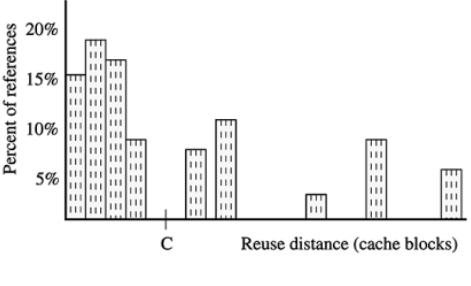
\includegraphics[width=4.91in,height=2.98in]{./media/image1.jpeg}
\end{figure}


%%%%%%%%%%%%%%%%%%%% Figure/Image No: 1 Ends here %%%%%%%%%%%%%%%%%%%%

\par


\vspace{\baselineskip}

\vspace{\baselineskip}

\vspace{\baselineskip}

\vspace{\baselineskip}

\vspace{\baselineskip}

\vspace{\baselineskip}

\vspace{\baselineskip}

\vspace{\baselineskip}

\vspace{\baselineskip}

\vspace{\baselineskip}

\vspace{\baselineskip}

\vspace{\baselineskip}

\vspace{\baselineskip}

\vspace{\baselineskip}

\vspace{\baselineskip}

\vspace{\baselineskip}

\vspace{\baselineskip}

\vspace{\baselineskip}

\vspace{\baselineskip}

\vspace{\baselineskip}

\vspace{\baselineskip}

\vspace{\baselineskip}

\vspace{\baselineskip}

\vspace{\baselineskip}

\vspace{\baselineskip}
{\fontsize{9pt}{10.8pt}\selectfont \textcolor[HTML]{666666}{Estimating reuse distance functions for each group. (a) Partitionings histogram into groups. (b) Pairing groups.}\par}\par


\vspace{\baselineskip}

\vspace{\baselineskip}
\begin{adjustwidth}{0.0in}{0.07in}
{\fontsize{10pt}{12.0pt}\selectfont \textcolor[HTML]{333333}{We justify this pairing of groups with observations that reuse patterns are a function of data size, \textit{s}, and this component dominates in determining the reuse distance. For a nontrivial data size, the result}\par}\par

\end{adjustwidth}


\vspace{\baselineskip}
\begin{adjustwidth}{0.0in}{0.18in}
{\fontsize{11pt}{13.2pt}\selectfont \textcolor[HTML]{333333}{is that the groups become sorted from left to right by functions of increasing power of \textit{s}, e.g., reuse distance increases more rapidly for groups based on \textit{s} than for those based on $ \surd$ s.}\par}\par

\end{adjustwidth}


\vspace{\baselineskip}
\begin{adjustwidth}{0.0in}{0.01in}
{\fontsize{10pt}{12.0pt}\selectfont \textcolor[HTML]{333333}{If we show three groups and the reuse distance histogram for two runs. In the second run, the movement of the groups is shown relative to the first run. The estimated function types are also shown. The first group, \textit{g}}{\fontsize{7pt}{8.4pt}\selectfont \textit{\textcolor[HTML]{333333}{i}}{\fontsize{10pt}{12.0pt}\selectfont \textcolor[HTML]{333333}{, does not move between the runs, so its reuse distance is independent of the data set size (\textit{constant}). On the other hand, \textit{g}}{\fontsize{7pt}{8.4pt}\selectfont \textit{\textcolor[HTML]{333333}{j}}{\fontsize{10pt}{12.0pt}\selectfont \textcolor[HTML]{333333}{ has a square root relationship to the data size, O($ \surd$ s) and \textit{g}}{\fontsize{7pt}{8.4pt}\selectfont \textit{\textcolor[HTML]{333333}{k}}{\fontsize{10pt}{12.0pt}\selectfont \textcolor[HTML]{333333}{ has a linear relationship, \textit{O(s)}. Dividing the histogram into 1, 000 groups limits the error from any single estimated model. The final model is a parameterized set of 1, 000 functions.}\par}\par}\par}\par}\par}\par}\par}\par

\end{adjustwidth}


\vspace{\baselineskip}
\begin{adjustwidth}{0.07in}{0.0in}
{\fontsize{18pt}{21.6pt}\selectfont Identifying Individual Patterns\par}\par

\end{adjustwidth}


\vspace{\baselineskip}
\begin{adjustwidth}{0.0in}{0.12in}
{\fontsize{10pt}{12.0pt}\selectfont \textcolor[HTML]{333333}{Given two histograms with different data sizes, the pattern recognition step constructs a formula for each group of references. Let d1i be the distance of the ith group in the first histogram, d2i be the distance of the ith group in the second histogram, \textit{s}}{\fontsize{7pt}{8.4pt}\selectfont \textit{\textcolor[HTML]{333333}{1}}{\fontsize{10pt}{12.0pt}\selectfont \textcolor[HTML]{333333}{ be the data size of the first run, and \textit{s}}{\fontsize{7pt}{8.4pt}\selectfont \textit{\textcolor[HTML]{333333}{2}}{\fontsize{10pt}{12.0pt}\selectfont \textcolor[HTML]{333333}{ the data size of the second run. The pattern for this group is a linear fitting based on the data size. Specifically, we want to find the two coefficients, \textit{c}}{\fontsize{7pt}{8.4pt}\selectfont \textit{\textcolor[HTML]{333333}{i}}{\fontsize{10pt}{12.0pt}\selectfont \textcolor[HTML]{333333}{ and \textit{e}}{\fontsize{7pt}{8.4pt}\selectfont \textit{\textcolor[HTML]{333333}{i}}{\fontsize{10pt}{12.0pt}\selectfont \textcolor[HTML]{333333}{, that satisfy the following two equations:}\par}\par}\par}\par}\par}\par}\par}\par}\par}\par

\end{adjustwidth}


\vspace{\baselineskip}
{\fontsize{11pt}{13.2pt}\selectfont \textcolor[HTML]{333333}{d1i=ci+ei$\ast$ fi(s1).(1)}\par}\par


\vspace{\baselineskip}
{\fontsize{11pt}{13.2pt}\selectfont \textcolor[HTML]{333333}{d2i=ci+ei$\ast$ fi(s2).(2)}\par}\par


\vspace{\baselineskip}

\vspace{\baselineskip}
\begin{adjustwidth}{0.0in}{0.01in}
{\fontsize{11pt}{13.2pt}\selectfont \textcolor[HTML]{333333}{Assuming the function fi is known, the two coefficients uniquely determine the distance for any other data size. The pattern is more accurate if more profiles are collected for the linear fitting. The minimal number of inputs is two.}\par}\par

\end{adjustwidth}


\vspace{\baselineskip}
\begin{adjustwidth}{0.0in}{0.08in}
{\fontsize{10pt}{12.0pt}\selectfont \textcolor[HTML]{333333}{The formula is based on an important fact about reuse distance: In any program, the largest reuse distance cannot exceed the size of program data. Therefore, the function fi can be linear at most, so the pattern is a linear or sublinear function of data size and not a general polynomial function. Following are the choices for fi : The first is pconst(s) = 0. A constant formula pattern because reuse distance does not change with data size. The second is plinear(s) = s, a linear pattern. The constant and linear patterns are the lower and upper bounds of the distance patterns. Between them are sublinear patterns.For each group pair (g1i,g2i), we calculate the ratio of their average distance, d2i/d1i, and pick fi to be the pattern function, p, such that p(s2)/p(s1) is closest to d2i/d1i.}\par}\par

\end{adjustwidth}


\vspace{\baselineskip}
\begin{adjustwidth}{0.0in}{0.1in}
{\fontsize{10pt}{12.0pt}\selectfont \textcolor[HTML]{333333}{According to the regression theory, more data can reduce the effect of noise and reveal a pattern closer to the true pattern . Using more than two training inputs in the analysis may produce a better prediction because it reduces the noise from imprecise reuse distance measurement and}\par}\par

\end{adjustwidth}


\vspace{\baselineskip}
\begin{adjustwidth}{0.0in}{0.01in}
{\fontsize{11pt}{13.2pt}\selectfont \textcolor[HTML]{333333}{reference histogram construction .The extension is straightforward. For each input, there is an equation as shown. For each bin, instead of two linear equations for two unknowns, there are as many equations as the number of training runs. Although more training data can lead to better results, they also lengthen the profiling process.}\par}\par

\end{adjustwidth}


\vspace{\baselineskip}
\begin{adjustwidth}{2.6in}{0.0in}
{\fontsize{11pt}{13.2pt}\selectfont \textcolor[HTML]{333333}{di=ci+ei$\ast$ fi(s)}\par}\par

\end{adjustwidth}



%%%%%%%%%%%%%%%%%%%% Figure/Image No: 2 starts here %%%%%%%%%%%%%%%%%%%%

\begin{figure}[H]
\advance\leftskip 0.02in		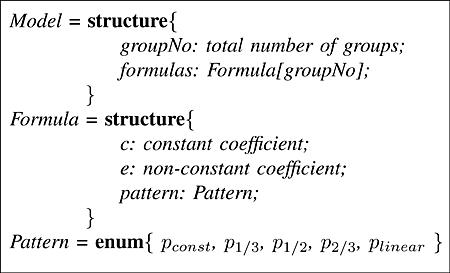
\includegraphics[width=4.31in,height=2.24in]{./media/image2.jpeg}
\end{figure}


%%%%%%%%%%%%%%%%%%%% Figure/Image No: 2 Ends here %%%%%%%%%%%%%%%%%%%%

\par


\vspace{\baselineskip}

\vspace{\baselineskip}

\vspace{\baselineskip}

\vspace{\baselineskip}

\vspace{\baselineskip}

\vspace{\baselineskip}

\vspace{\baselineskip}

\vspace{\baselineskip}

\vspace{\baselineskip}

\vspace{\baselineskip}

\vspace{\baselineskip}

\vspace{\baselineskip}

\vspace{\baselineskip}

\vspace{\baselineskip}

\vspace{\baselineskip}

\vspace{\baselineskip}

\vspace{\baselineskip}

\vspace{\baselineskip}
{\fontsize{11pt}{13.2pt}\selectfont \textcolor[HTML]{333333}{Here p1/3,p1/2,p2/3 are sub linear functions of s .ex. p2/3(s)=s$ \string^ $ ⅔.}\par}\par


\vspace{\baselineskip}

\vspace{\baselineskip}
{\fontsize{16pt}{19.2pt}\selectfont Cache Miss Rate Estimation from predicted reuse distances\par}\par


\vspace{\baselineskip}
\begin{adjustwidth}{0.0in}{0.17in}
{\fontsize{10pt}{12.0pt}\selectfont \textcolor[HTML]{333333}{After generating the locality model of a program, locality behavior for any data input size \textit{s can be} \textit{predicted }. The reuse distance for each group\textit{ g}}{\fontsize{7pt}{8.4pt}\selectfont \textit{\textcolor[HTML]{333333}{i}}{\fontsize{10pt}{12.0pt}\selectfont \textit{\textcolor[HTML]{333333}{ }}\textcolor[HTML]{333333}{can be predicted via their particular formula. The\textit{ }overall reuse distance distribution is the aggregation of the reuse distance of each group. For any given size of a fully associative LRU cache, the capacity miss rate is directly estimated from the reuse distance distribution. The groups with a reuse distance larger than or equal to the given cache size will be capacity misses. The number of these groups gives an estimate of the miss rate. The}\par}\par}\par}\par

\end{adjustwidth}


\vspace{\baselineskip}


%%%%%%%%%%%%%%%%%%%% Figure/Image No: 3 starts here %%%%%%%%%%%%%%%%%%%%

\begin{figure}[H]
	\begin{Center}
		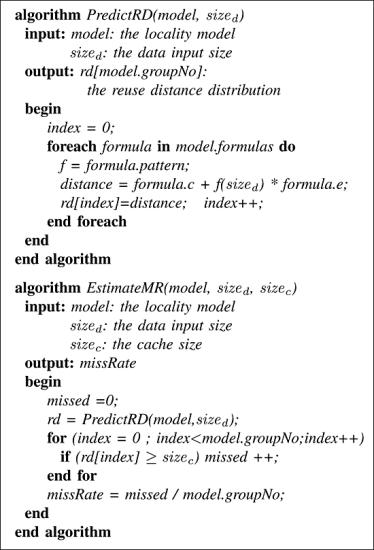
\includegraphics[width=3.9in,height=5.73in]{./media/image3.jpeg}
	\end{Center}
\end{figure}


%%%%%%%%%%%%%%%%%%%% Figure/Image No: 3 Ends here %%%%%%%%%%%%%%%%%%%%

\begin{adjustwidth}{0.0in}{0.38in}
{\fontsize{11pt}{13.2pt}\selectfont \textcolor[HTML]{333333}{detailed algorithms for reuse distance prediction and cache miss rate estimation are described as follows }\par}\par

\end{adjustwidth}


\vspace{\baselineskip}
\begin{adjustwidth}{0.0in}{0.01in}
{\fontsize{10pt}{12.0pt}\selectfont \textcolor[HTML]{333333}{From our locality model, we can also derive the maximum possible miss rate of a program for a given cache size. Here, we consider two important properties of the reuse distance model. First, only references with a reuse distance larger than or equal to the cache size are cache misses. References with a shorter reuse distance will hit in cache because of temporal locality. The second property is that reuse distances of references having linear or sublinear patterns monotonically increase with the input size. The distances of references having a constant pattern, on the other hand, are independent of the input size. From these two facts, we can infer that, for a certain cache size, if we increase the program data input size, the cache miss rate may remain the same or increase, but it will never decrease. Furthermore, the maximum miss rate will be reached when the input size is large enough so that all references with a nonconstant pattern have a reuse distance larger than the cache size.}\par}\par

\end{adjustwidth}


\vspace{\baselineskip}
\begin{adjustwidth}{0.0in}{0.04in}
{\fontsize{11pt}{13.2pt}\selectfont \textcolor[HTML]{333333}{Figure below shows the main algorithm to predict the maximum cache miss rate and the corresponding threshold input size for a given cache of \textit{size}}{\fontsize{7pt}{8.4pt}\selectfont \textit{\textcolor[HTML]{333333}{c}}{\fontsize{11pt}{13.2pt}\selectfont \textcolor[HTML]{333333}{ blocks. Suppose, among the total \textit{G} groups (\textit{G = 1, 000} for all our results), the number of reference groups with a pattern dependent on data size \textit{s} is \textit{G}}{\fontsize{7pt}{8.4pt}\selectfont \textit{\textcolor[HTML]{333333}{s}}{\fontsize{11pt}{13.2pt}\selectfont \textcolor[HTML]{333333}{ and the number of groups having a pattern independent of data size (constant) with a fixed reuse distance greater than the capacity of the cache is}\par}\par}\par}\par}\par}\par

\end{adjustwidth}



%%%%%%%%%%%%%%%%%%%% Figure/Image No: 4 starts here %%%%%%%%%%%%%%%%%%%%

\begin{figure}[H]
\advance\leftskip 0.02in		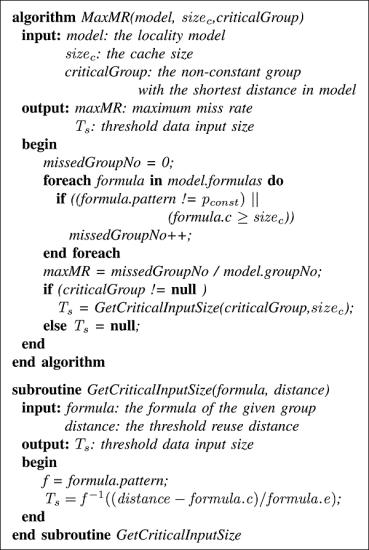
\includegraphics[width=3.55in,height=4.57in]{./media/image4.jpeg}
\end{figure}


%%%%%%%%%%%%%%%%%%%% Figure/Image No: 4 Ends here %%%%%%%%%%%%%%%%%%%%

\par


\vspace{\baselineskip}

\vspace{\baselineskip}

\vspace{\baselineskip}

\vspace{\baselineskip}

\vspace{\baselineskip}

\vspace{\baselineskip}

\vspace{\baselineskip}

\vspace{\baselineskip}

\vspace{\baselineskip}

\vspace{\baselineskip}

\vspace{\baselineskip}

\vspace{\baselineskip}

\vspace{\baselineskip}

\vspace{\baselineskip}

\vspace{\baselineskip}

\vspace{\baselineskip}

\vspace{\baselineskip}

\vspace{\baselineskip}

\vspace{\baselineskip}

\vspace{\baselineskip}

\vspace{\baselineskip}

\vspace{\baselineskip}

\vspace{\baselineskip}

\vspace{\baselineskip}

\vspace{\baselineskip}

\vspace{\baselineskip}

\vspace{\baselineskip}

\vspace{\baselineskip}

\vspace{\baselineskip}

\vspace{\baselineskip}

\vspace{\baselineskip}

\vspace{\baselineskip}

\vspace{\baselineskip}

\vspace{\baselineskip}
{\fontsize{8pt}{9.6pt}\selectfont \textbf{\textcolor[HTML]{666666}{Fig. 5. }}\textcolor[HTML]{666666}{Max miss rate and threshold input prediction.}\par}\par


\vspace{\baselineskip}

\vspace{\baselineskip}
\begin{adjustwidth}{0.04in}{0.0in}
{\fontsize{11pt}{13.2pt}\selectfont \textit{\textcolor[HTML]{333333}{G}}{\fontsize{8pt}{9.6pt}\selectfont \textit{\textcolor[HTML]{333333}{c}}{\fontsize{11pt}{13.2pt}\selectfont \textcolor[HTML]{333333}{, the maximum miss rate is calculated as\textit{ Miss Rate}}{\fontsize{8pt}{9.6pt}\selectfont \textit{\textcolor[HTML]{333333}{max}}{\fontsize{11pt}{13.2pt}\selectfont \textit{\textcolor[HTML]{333333}{ = (G}}{\fontsize{8pt}{9.6pt}\selectfont \textit{\textcolor[HTML]{333333}{s}}{\fontsize{11pt}{13.2pt}\selectfont \textit{\textcolor[HTML]{333333}{ + G}}{\fontsize{8pt}{9.6pt}\selectfont \textit{\textcolor[HTML]{333333}{c}}{\fontsize{11pt}{13.2pt}\selectfont \textit{\textcolor[HTML]{333333}{)/G}}\textcolor[HTML]{333333}{.}\par}\par}\par}\par}\par}\par}\par}\par}\par}\par

\end{adjustwidth}


\vspace{\baselineskip}

\vspace{\baselineskip}
\begin{adjustwidth}{0.0in}{0.01in}
{\fontsize{10pt}{12.0pt}\selectfont \textcolor[HTML]{333333}{The \textit{threshold input size (T}}{\fontsize{7pt}{8.4pt}\selectfont \textit{\textcolor[HTML]{333333}{s}}{\fontsize{10pt}{12.0pt}\selectfont \textit{\textcolor[HTML]{333333}{)}}\textcolor[HTML]{333333}{ is the smallest input size in which the cache miss rate reaches the maximum value for the program and the given cache configuration. To estimate its value, we only need to consider the single non constant reference group having the shortest reuse distance. The maximum miss rate occurs when this group, \textit{g}}{\fontsize{7pt}{8.4pt}\selectfont \textit{\textcolor[HTML]{333333}{j}}{\fontsize{10pt}{12.0pt}\selectfont \textcolor[HTML]{333333}{, has a reuse distance greater than or equal to the cache size, \textit{d}}{\fontsize{7pt}{8.4pt}\selectfont \textit{\textcolor[HTML]{333333}{j}}{\fontsize{10pt}{12.0pt}\selectfont \textcolor[HTML]{333333}{ \textit{$ \geq $  size}}{\fontsize{7pt}{8.4pt}\selectfont \textit{\textcolor[HTML]{333333}{c}}{\fontsize{10pt}{12.0pt}\selectfont \textcolor[HTML]{333333}{.We can directly calculate the required input data size from this condition:}\par}\par}\par}\par}\par}\par}\par}\par}\par}\par

\end{adjustwidth}


\vspace{\baselineskip}

\vspace{\baselineskip}
\begin{adjustwidth}{1.64in}{0.0in}
\textcolor[HTML]{333333}{T}{\fontsize{8pt}{9.6pt}\selectfont \textcolor[HTML]{333333}{s=f(-1)j((C$-$ cj)/ej).(4)}\par}\par

\end{adjustwidth}


\vspace{\baselineskip}
\begin{adjustwidth}{0.0in}{0.07in}
{\fontsize{10pt}{12.0pt}\selectfont \textcolor[HTML]{333333}{If the model only contains the constant pattern, the cache miss rate is the same for all inputs. In this case, \textit{e}}{\fontsize{7pt}{8.4pt}\selectfont \textit{\textcolor[HTML]{333333}{j}}{\fontsize{10pt}{12.0pt}\selectfont \textcolor[HTML]{333333}{ is zero and generates a meaningless null threshold input. The threshold input size \textit{T}}{\fontsize{7pt}{8.4pt}\selectfont \textit{\textcolor[HTML]{333333}{s}}{\fontsize{10pt}{12.0pt}\selectfont \textcolor[HTML]{333333}{ is useful since it is the smallest input that generates the worst case hit ratio for a fully associative cache.}\par}\par}\par}\par}\par}\par

\end{adjustwidth}


\vspace{\baselineskip}
\begin{adjustwidth}{0.0in}{0.07in}
{\fontsize{10pt}{12.0pt}\selectfont \textit{\textcolor[HTML]{333333}{Model accuracy verification:}}\textcolor[HTML]{333333}{Only two input sets are necessary to generate a miss rate model for a\textit{ }program. However, if more input sets are measured, multiple models can be generated from pairwise groupings and the predictions evaluated for the excluded data set sizes. For example, for three data set sizes, \textit{A}, \textit{B}, and \textit{C}, three combinations of pairs are possible, \textit{(A, B)}, \textit{(A, C)}, and \textit{(B, C)}. The data sets used for verification would be \textit{C}, \textit{B}, and \textit{A}, respectively. Thus, a degree of confidence for the model can be measured with limited exploration of the data set space.}\par}\par

\end{adjustwidth}


\vspace{\baselineskip}

\vspace{\baselineskip}

\vspace{\baselineskip}

\vspace{\baselineskip}
{\fontsize{20pt}{24.0pt}\selectfont \textbf{References}\par}\par


\vspace{\baselineskip}

\vspace{\baselineskip}
\begin{adjustwidth}{0.0in}{0.15in}
{\fontsize{10pt}{12.0pt}\selectfont 1)Y. Zhong, S. Dropsho, and C. Ding.$``$Miss Rate Prediction Across Program Inputs and Cache Configurations$"$ ,IEEE TRANSACTIONS ON COMPUTERS, VOL. 56, NO. 3, MARCH 2007.\par}\par

\end{adjustwidth}


\vspace{\baselineskip}
\begin{adjustwidth}{0.0in}{0.43in}
{\fontsize{11pt}{13.2pt}\selectfont 2)Changpeng Fang , Steve Carr ,Soner Onder and Zhenlin Wang$"$  Reuse-distance-based Miss-rate Prediction on a Per Instruction Basis$"$ \par}\par

\end{adjustwidth}


\vspace{\baselineskip}
\begin{adjustwidth}{0.0in}{0.22in}
{\fontsize{11pt}{13.2pt}\selectfont 3)C. Ding and Y. Zhong, $``$Predicting Whole-Program Locality with Reuse Distance Analysis,$"$  Proc. ACM SIGPLAN Conf. Programming Language Design and Implementation, June 2003.\par}\par

\end{adjustwidth}


\printbibliography
\end{document}
